\documentclass{article}

\usepackage[a4paper,landscape,margin=2cm]{geometry}
\usepackage{../../../../components/mathtex}
\usepackage{colortbl}
\usepackage{array}

\usepackage{fancyhdr}
\usepackage{ulem}
\usepackage{paracol}

\pagestyle{fancy}
\fancyhf{}
\fancyhead[L]{DL3 Math-Info}
\fancyhead[C]{Fiche d'entraînement hebdomadaire N°4}
\fancyhead[R]{2026-2027}
\fancyfoot[L]{Ewen Rodrigues de Oliveira}
\fancyfoot[R]{\thepage}


\begin{document}
\setlength{\columnsep}{2cm}

\begin{paracol}{2}

\renewcommand{\arraystretch}{1.3}
\noindent
\begin{tabular}{|p{0.6\columnwidth}|>{\centering\arraybackslash}p{0.35\columnwidth}|}
\hline
\rowcolor[RGB]{230,237,247}
\textbf{Matière} & \textbf{Exercices} \\
\hline
Intégration et probabilités & $5,6,7,8,9,10$\\
\hline
Groupes et actions & $11,12,13,14,15$\\
\hline
Calcul différentiel & $1,2,3,4$\\
\hline
Systèmes d'exploitation & $\emptyset$\\
\hline
Algorithmique & $16$\\
\hline
Programmation fonctionnelle & $\emptyset$\\
\hline
Anglais & $\emptyset$\\
\hline
\end{tabular}

\vspace{1em}

\exercise{1}{Équivalence de normes}{
    Soit $E = \mathbb{R}[X]$ l'espace vectoriel des polynômes à coefficients réels.  
Pour tout polynôme $P = \sum_{k=0}^n a_k X^k \in E$, on définit :
\begin{enumerate}
    \item $\|P\|_1 = \sum_{k=0}^n |a_k|$
    \item $\|P\|_\infty = \sup_{t \in [0, 1]} |P(t)|$
\end{enumerate}

On admet que $\|\cdot\|_1$ et $\|\cdot\|_\infty$ sont des normes sur $E$.
Les normes $\|\cdot\|_1$ et $\|\cdot\|_\infty$ sont-elles équivalentes sur $E$?
}

\exercise{2}{Étude de la continuité}{
    Les applications suivantes sont-elles continues sur leurs domaines respectifs?
    \begin{enumerate}
        \item $f : (\mathbb{R}^2, \|\cdot\|_2) \to (\mathbb{R}, |\cdot|)$ donnée par $f(x_1, x_2) = x_1^2 + x_2^2$.
        \item $f : (\mathbb{R}^n, \|\cdot\|_1) \to (\mathbb{R}, |\cdot|)$ donnée par $f(x_1, \dots, x_n) = \displaystyle\sum_{k=1}^n x_k$.
        \item $f : (\mathbb{R}^2, \|\cdot\|_2) \to (\mathbb{R}^2, \|\cdot\|_2)$ donnée par $f(x, y) = \left(x^2 y, \dfrac{y + x^3}{1 + x^2}\right)$.
        \item $f : (\mathbb{R}^2, \|\cdot\|_2) \to (\mathbb{R}^2, \|\cdot\|_2)$ donnée par $f(x) = Ax$, avec $A = \begin{pmatrix} 2 & 1 \\ 1 & 2 \end{pmatrix}$.
        \item $f : \mathbb{R}^2 \to \mathbb{R}$ donnée par 
        \[
            f(x, y) = \begin{cases} \dfrac{xy}{x^2 + y^2} & \text{si } (x, y) \neq (0, 0) \\ 0 & \text{sinon.} \end{cases}
        \]
    \end{enumerate}
}

\switchcolumn

\exercise{3}{Fonctions uniformément continues sur $\mathbb{R}$}{
    Soient $\alpha \in {]0, 1[}$ et $f : \mathbb{R}^+ \to \mathbb{R}^+$ donnée par
    \[
    f(x) = x^\alpha.
    \]
    \begin{enumerate}
        \item Montrer que $f$ est uniformément continue sur $[0, +\infty[$ pour $\alpha = 1/2$.
        \item Montrer que $f$ est lipschitzienne sur $[a, +\infty[$ pour tout $a > 0$ et calculer la constante de Lipschitz.
        \item Montrer que $f$ n'est pas lipschitzienne sur $[0, +\infty[$.
    \end{enumerate}
}

\exercise{4}{Fonctions lipschitziennes sur $\mathbb{R}^2$}{
    Considérons l'application $f : \mathbb{R}^2 \to \mathbb{R}$, donnée par
    \[
    f(x,y) = 2x - 3y
    \]
    \begin{enumerate}
        \item Considérant que $\mathbb{R}^2$ est muni de la norme $\|\cdot\|_2$, cette application est-elle Lipschitzienne ? Si oui, calculer la constante de Lipschitz correspondante.
        \item Reprendre cette question avec la norme $\|\cdot\|_1$, puis $\|\cdot\|_\infty$.
    \end{enumerate}
}

\exercise{5}{Probabilités conditionnelles et urnes}{
    On considère 3 urnes :
    \begin{itemize}
        \item U1 contient 2 boules noires et 3 rouges.
        \item U2 contient 1 boule noire et 4 rouges.
        \item U3 contient 3 boules noires et 4 rouges.
    \end{itemize}
    On tire, uniformément, une boule dans U1 et une boule dans U2, et on les met dans U3.
    On tire une boule de U3, elle est noire. Quelle est la probabilité que la boule tirée de U1 soit rouge ?
}

\exercise{6}{Préparation du CM}{Passer le QCM "Rappels de cours 1" sur la page Moodle de Intégration et Probabilités.}

\switchcolumn
\newpage
\exercise{7}{Caractérisation de mesures et de probabilités}{
    On liste ci-dessous des applications $\mu : \mathcal{B}(\mathbb{R}) \to \mathbb{R}_+ \cup \{+\infty\}$, en exprimant $\mu(A), A \in \mathcal{B}(\mathbb{R})$. Déterminer lesquelles sont des mesures positives et/ou des mesures de probabilité sur $(\mathbb{R}, \mathcal{B}(\mathbb{R}))$. On justifiera la réponse.
    \begin{enumerate}
        \item Pour tout $A \in \mathcal{B}(\mathbb{R})$, $\mu(A) = \sum_{k=-5}^5 k \mathbf{1}_{\{k \in A\}}$,
        \item Pour tout $A \in \mathcal{B}(\mathbb{R})$, $\mu(A) = \sum_{k \ge 0} 2^{-k} \mathbf{1}_{\{k \in A\}}$,
        \item Pour tout $A \in \mathcal{B}(\mathbb{R})$, $\mu(A) = \sum_{k \ge 1} 2^{-k} \mathbf{1}_{\{4-k \in A\}}$,
        \item Pour tout $A \in \mathcal{B}(\mathbb{R})$, $\mu(A) = \frac{8}{15} + \frac{4}{15} \sum_{k \ge 1} \frac{(\ln(3))^k}{k!} \mathbf{1}_{\{k \in A\}}$,
    \end{enumerate}
}

\exercise{8}{Manipulation de l'intégrale de Lebesgue}{
    Soit $E = [0, 3]$ muni de sa tribu borélienne $\mathcal{B}([0, 3])$.
On considère la fonction mesurable positive $f : [0, 3] \to \mathbb{R}_+$ définie par :
$$f(x) = \begin{cases} 
2 & \text{si } x \in [0, 1[ \\ 
x^2 & \text{si } x \in [1, 3] 
\end{cases}$$

Calculer l'intégrale $\int_{[0, 3]} f \, d\mu$ dans chacun des cas suivants :
\begin{enumerate}
    \item $\mu = \delta_0$ (la mesure de Dirac au point $0$).
    \item $\mu = \delta_2$ (la mesure de Dirac au point $2$).
    \item $\mu = 3 \delta_0 + 2 \delta_2$.
    \item $\mu = \lambda$ (la mesure de Lebesgue sur $[0, 3]$).
\end{enumerate}
}
\exercise{9}{Recherche de constantes de normalisation}{
    Dans les cas suivants, trouver la valeur de $C$ pour que $f$ soit une densité de probabilité.
    \begin{enumerate}
        \item $f(x) = \frac{C}{\sqrt{x(1-x)}}$, $0 < x < 1$. \textit{(indication : on pourra effectuer le changement de variables $u = \sqrt{x}$)}
        \item $f(x) = C \exp(-x - \exp(-x))$, $x \in \mathbb{R}$,
        \item $f(x) = C \frac{1}{1+x^2}$
    \end{enumerate}
}
\switchcolumn
\newpage
\exercise{10}{Intégration d'une fonction étagée}{
    On se place sur $E = [-1, 2]$ muni de la mesure de Lebesgue $\lambda$.
    On considère l'application $g : [-1, 2] \to \mathbb{R}_+$ définie par :
    $$g(x) = \begin{cases} 
    3 & \text{si } x \in [-1, 0] \setminus \{ -1/2 \} \\ 
    0 & \text{si } x = -1/2 \\ 
    1 & \text{si } x \in ]0, 2] 
    \end{cases}$$

    \begin{enumerate}
        \item Quelles sont les valeurs distinctes prises par la fonction $g$ ?
        \item Déterminer explicitement les ensembles $A_i \in \mathcal{B}([-1, 2])$ associés à chaque valeur distincte $\alpha_i$.
        \item Réécrire $g$ sous sa forme étagée canonique $g = \sum_{i=1}^n \alpha_i \mathbf{1}_{A_i}$.
        \item En justifiant avec la $\sigma$-additivité de la mesure de Lebesgue, calculer $\lambda(A_i)$ pour chaque ensemble $A_i$.
        \item En déduire la valeur de l'intégrale $\int_{[-1, 2]} g \, d\lambda$.
    \end{enumerate}
}

\exercise{11}{Relations d'équivalence}{
    Soit $E$ un ensemble. Soit $\mathcal{R}$ une relation binaire sur $E$. Dans chacun des cas suivants, déterminer si $\mathcal{R}$ est une relation d'équivalence. Le cas échéant, décrire les classes d'équivalence.
    \begin{enumerate}
        \item $E = \mathbb{N}$ et : $(\forall x,y \in E) \quad x\mathcal{R}y \iff x = -y$.
        \item $E = \mathbb{R}$ et : $(\forall x,y \in E) \quad x\mathcal{R}y \iff \cos^2 x + \sin^2 y = 1$.
        \item $E = \mathbb{R}$ et $(\forall x,y \in E) \quad x\mathcal{R}y \iff \lfloor x \rfloor = \lfloor y \rfloor$.
        \item $E = \{1, 2, 3\}$ et $\mathcal{R}$ est de graphe $\{(1, 1), (1, 2), (1, 3), (2, 1), (2, 2), (3, 1), (3, 3)\}$.
    \end{enumerate}
}

\exercise{12}{Relation sur $\mathbb{N} \times \mathbb{N}$}{
    On note $\mathcal{R}$ la relation binaire sur $\mathbb{N} \times \mathbb{N}$ définie par :
    \[
    \forall(a,b) \in \mathbb{N} \times \mathbb{N}, \quad \forall(a',b') \in \mathbb{N} \times \mathbb{N}, \quad (a,b)\,\mathcal{R}\,(a',b') \iff a + b' = a' + b.
    \]
    \begin{enumerate}
        \item Démontrer que $\mathcal{R}$ est une relation d'équivalence.
        \item Décrire les classes d'équivalence.
    \end{enumerate}
}
\switchcolumn
\newpage

\exercise{13}{Congruence dans $\mathbb{R}[X]$}{
    Soit $B \in \mathbb{R}[X]$, $B \neq 0$. On note $\mathcal{R}$ la relation binaire sur $\mathbb{R}[X]$ définie par : $\forall A, A' \in \mathbb{R}[X], \quad A\mathcal{R}A' \iff B \mid (A - A')$.
    \begin{enumerate}
        \item Démontrer que $\mathcal{R}$ est une relation d'équivalence.
        \item Soit $A \in \mathbb{R}[X]$. Décrire la classe d'équivalence de $A$.
        \item Démontrer qu'il existe une application de $\mathbb{R}[X]/\mathcal{R}$ dans $\mathbb{R}_{\deg(B)-1}[X]$ telle que, pour tout $A \in \mathbb{R}[X]$, l'image de la classe d'équivalence de $A$ par cette application soit le reste de la division euclidienne de $A$ par $B$.
        \item Démontrer que l'application obtenue à la question précédente est bijective.
    \end{enumerate}
}

\exercise{14}{Relation de même module sur $\mathbb{C}$}{
    On note $\mathcal{R}$ la relation binaire sur $\mathbb{C}$ définie par :
    \[
    \forall z, z' \in \mathbb{C}, \quad z\mathcal{R}z' \iff |z| = |z'|
    \]
    \begin{enumerate}
        \item Démontrer que $\mathcal{R}$ est une relation d'équivalence.
        \item Soit $z \in \mathbb{C}$. Décrire la classe d'équivalence de $z$ à l'aide de l'écriture exponentielle des nombres complexes. La représenter sur un dessin.
        \item Démontrer qu'il existe une application de $\mathbb{C}/\mathcal{R}$ dans $\mathbb{R}_+$ telle que, pour tout $z \in \mathbb{C}$, l'image de la classe d'équivalence de $z$ par cette application soit $|z|$.
        \item Démontrer que l'application obtenue à la question précédente est bijective.
    \end{enumerate}
}

\exercise{15}{Invariants par isomorphisme de groupes}{
    Soient $G$ et $H$ deux groupes isomorphes. Prouver les affirmations suivantes.
    \begin{enumerate}
        \item $G$ est abélien si et seulement si $H$ est abélien.
        \item $G$ est monogène si et seulement si $H$ est monogène.
    \end{enumerate}
    On suppose de plus que les groupes $G$ et $H$ sont finis. Prouver que
    \begin{enumerate}
        \setcounter{enumi}{2}
        \item Pour tout $n \in \mathbb{N}^*$, les groupes $G$ et $H$ ont le même nombre d'éléments d'ordre $n$.
        \switchcolumn
        \item $G$ est cyclique si et seulement si $H$ est cyclique.
        \item $G$ et $H$ ont le même nombre de sous-groupes.
        \setcounter{enumi}{0}
    \end{enumerate}
}

\exercise{16}{Parcours en Profondeur}{
    \begin{enumerate}
        \item Exécuter un parcours en profondeur sur le graphe de la figure 1. Donnez les dates de pré- et post-visite pour chaque sommet, ainsi que l'arbre du parcours. Considérer que les listes d'adjacence sont données en ordre alphabétique croissant des sommets.
        \item Y a-t-il une exécution de parcours en profondeur sur le graphe de la figure 1 telle que il n'y a pas d'arc de type retour ? Justifier votre réponse.
        \item Le graphe de la figure 1 admet-il un tri topologique ? Si oui, donner un tri valide, sinon expliquer pourquoi.
        \item Trouver les sources et les puits du graphe de la figure 1.
        \item On a déjà exécuté un parcours en profondeur sur le graphe de la figure 2 qui départ du sommet en haut à gauche. On vous donne l'arbre du parcours (les arcs du parcours sont en gras). Donnez les types des 10 autres arcs et les dates de pré- et post-visite correspondant à cet arbre de parcours.
    \end{enumerate}

    \begin{center}
    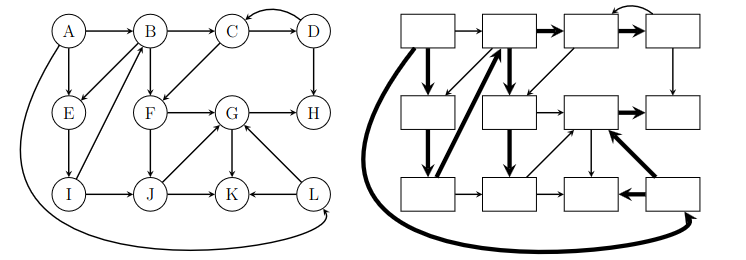
\includegraphics[width=0.5\textwidth]{./algo.png}

    \end{center}
}

\end{paracol}
\end{document}